\documentclass[a4paper,11pt]{report}
\usepackage[utf8]{inputenc}
\usepackage[T1]{fontenc}
\usepackage[utf8]{inputenc}
\usepackage{lmodern}
\usepackage[french]{babel}
\usepackage{varioref}
\usepackage{numprint}
\usepackage{multirow}
\usepackage{caption}
\usepackage{hyperref}
\usepackage[toc]{glossaries}
\usepackage{pgf,tikz}
\usepackage{graphicx}
%\usepackage{parskip}
%\usepackage{syntax}

\title{Nauteff-Vision Spécification}
\author{Emmanuel \textsc{Gautier}}


%%\newglossaryentry{MEMS}{name=Nom, description={}}

\newglossaryentry{babord} {
	name=bâbord,
	sort={BABORD},
	description={désigne le côté gauche d'un navire, en tournant le dos à la poupe}
}

\newglossaryentry{tribord} {
	name=tribord,
	description={le côté droit d'un navire, en tournant le dos à la poupe}
}

\newglossaryentry{cavalement} {
	name=cavalement,
	sort={CAVALEMENT},
	description={Mouvement le long de l'axe longitudinal du navire, c.à.d. d'avant en arrière, ce mouvement correspond à une accélération ou un ralentissement.}
}

\newglossaryentry{embardee} {
	name=embardée,
	sort={EMBARDEE},
	description={Mouvement latéral du navire, c.à.d. vers son côté. Il est souvent provoqué par les rafales de vent et la houle. Il est souvent liée à la gîte et à la dérive}
}

\newglossaryentry{I2C} {
	name=I2C,
	description={Inter-Integrated Circuit en englais. C'est un bus de communication série à 2 fils à courte distance.}
}

\newglossaryentry{gite} {
	name=gîte,
	description={inclinaison latérale d'un navire. La gîte est généralement due au vent.}
}

\newglossaryentry{MEMS} {
    name=MEMS,
    description={Micro Electro Mechanicals Systems ou, en français, systèmes micro électromécaniques. Parmi ces systèmes figurent le magnétomètre, l'accéléromètre et le gyromètre.}
    }

\newglossaryentry{NMEA}
{
	name={NMEA}, % le terme à référencer (l'entrée qui apparaitra dans le glossaire)
	description={National Marine Electronics Association. Cet organisme américain a créé les protocoles NMEA~0183 et NMEA~2000}, % la description du terme(sans retour à la ligne)
	sort={NMEA}, % si le mot contient des caractère spéciaux, ils ne seront pas pris en compte
	plural={NMEA} % la forme plurielle du terme
}

\newglossaryentry{NMEA0183}
{
	name={NMEA0183}, % le terme à référencer (l'entrée qui apparaitra dans le glossaire)
	description={Protocole Normalisé et non officiellement documenté défini par la NMEA utilisé par des appareils de navigation}, % la description du terme(sans retour à la ligne)
	sort={NMEA0183}, % si le mot contient des caractère spéciaux, ils ne seront pas pris en compte
	plural={NMEA0183} % la forme plurielle du terme
}

\newglossaryentry{pilonnement} {
    name=pilonnement,
    sort={PILONNEMENT},
    description={Mouvement vertical du navire, c.à.d. de bas en haut et de haut en bas. ce mouvement est généralement provoqué par les vagues.}
    }

\newglossaryentry{roulis} {
	name=roulis,
	description={ Mouvement d'oscillation d'un bateau autour de l'axe longitudinal (en général sous l'effet de la houle ou du vent)}
}

\newglossaryentry{quaternion} {
	name=quaternion,
	sort={QUATERNION},
	description={Nombre hypercomplexe formé par une partie réelle et 3 parties imaginaires, il servent à représenter l'orientation du navire}
}

\newglossaryentry{lacet} {
	name=lacet,
	description={mouvement de rotation par rapport à l'axe vertical du navire}
    }

\newglossaryentry{tangage} {
	name=Tangage,
	description={mouvement de rotation par rapport à l'axe transversal du navire}
    }

\newglossaryentry{UART} {
	name=UART,
	description={Universal Asynchronous Receiver Transmitter soit émetteur-récepteur asynchrone universel, aussi appelée liaison série.}
}


\makeglossaries
%\makeglossaries

\tikzset{every picture/.style={execute at begin picture={
			\shorthandoff{:;!?};}
}}

\newcommand{\myref}[1]{\ref{#1} p.\ \pageref{#1}}

\begin{document}
\maketitle

\begin{abstract}
Ce document contient la spécification du logiciel Nauteff-Vision.
\end{abstract}

\chapter*{Historique du document}
\begin{tabular}{|c|c|c|c|}
	\hline 
	Date & Évolutions & Version \\ 
	\hline
	27 août 2022 & Création du document  &  brouilon\\ 
    \hline 
    25 Juillet 2024 &    Reprise de la rédaction &brouillon\\
	\hline
\end{tabular} 
\tableofcontents
%\printglossary
\listoftables

\chapter{Buts du document}
\section{Buts}

C'est le document de référence décrivant
les exigences techniques et opérationnelles et la description
des fonctions du logiciel Nauteff-Vision.

Il est destiné aux acteurs participant
à la définition du système, à sa réalisation,
à sa mise au point et à ses essais.

Il complète le manuel d'utilisation en lui apportant des précisions.

\section{Guide de lecture}


Le chapitre \ref{presentation}, page\ \pageref{presentation}
fournit une description générale du logiciel dans son environnement.

Les annexes contiennent la description des données et des protocoles.
Bien que décrivant le système il n'est pas un manuel d'utilisation.
La rédaction du manuel d'utilisation n'est à ce jour pas encore commencée.
Le détail des fonctions de calculs et algorithmes est contenu
dans un autre document à venir.
Ce document sert de référence 
Nauteff-Vision est un complément du Nauteff-AP,
la lecture de la spécification de ce dernier est recommandée.

\section{Conventions typographiques}

\chapter{Documents applicables et de référence}

NMEA revealed : https://gpsd.gitlab.io/gpsd/NMEA.html
Ce document contient une description du protocole NMEA~0183.


%\chapter{Terminologie}
% \printglossary provoque l'affichage d'un chapitre
% avec le titre précisé par la directive title
%\printglossary[numberedsection, title=Terminologie]
\printglossary[numberedsection, type=\acronymtype, title=Terminologie]

\chapter{Présentation du logiciel}
\label{presentation}
Le graphique suivant présente l'environnement matériel et humain
de Nauteff-Vision à bord d'un navire ou au bureau.

% \section{graphique}
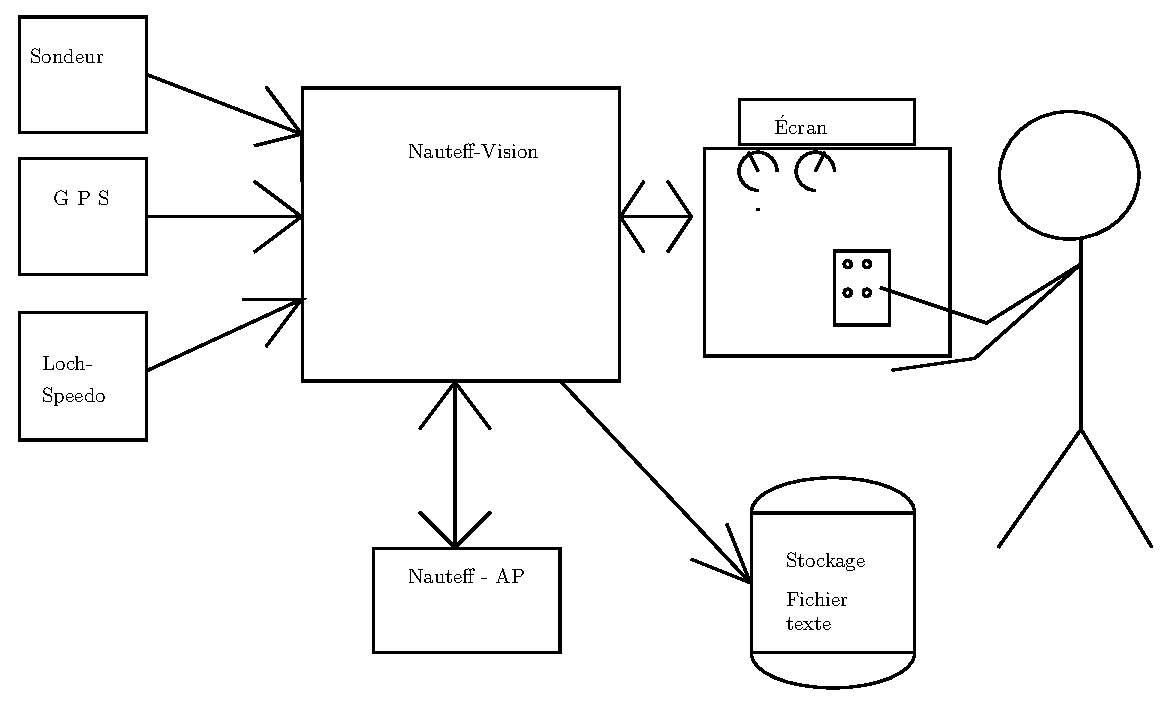
\includegraphics[width=10cm]{figures/Nauteff-Vision-envt.eps}


\section{Objectifs du logiciel}

Nauteff-Vision a été initialement destiné aux développeurs de Nauteff-AP,
et ensuite aussi aux navigateurs; ainsi ses objectifs sont :
\begin{itemize}
	\item Accéder au cœur de Nauteff-AP pour son développement et sa mise au point;
	\item Être une interface pour l'utilisateur du Nauteff-AP ;
	\item Aider le navigateur à mieux appréhender la conduite de son navire, en particulier pour l'apprentissage et l'entraînement;
	\item Apporter un accès libre et ouvert aux données de navigation et fonctions de calcul ou d'affichage;
	\item Enregistrer les données pour traitements et affichages ultérieurs;
	\item Expérimenter de nouveaux traitements sur les données;
	\item Être un outil de mise au point des systèmes de navigétion des navires.
\end{itemize}

\section{Environnement du logiciel}

Étant destiné au développement du Nauteff-AP et à l'aide à la navigation,
il est destiné à être utilisé dans un bureau ou à bord d'un navire.


Nauteff-Vision reçoit des données d'instruments de navigation et en transmet à ces instruments, en particulier au pilote automatique, il interagit avec un utilisateur et
enregistre des données dans un ou plusieurs fichiers.
Il relit aussi les données enregistrées, le traite et les affiche.

\subsection{Matériel}

Nauteff-Vision fonctionne sur les matériels suivants:
\begin{itemize}
	\item Nano-ordinateurs avec Linux ou Android;
    \item PC portables avec Linux ou Windows ;
    \item PC de bureau avec Linux ou Windows.
\end{itemize}

\subsection{Interfaces}

Les interfaces de Nauteff-Vision sont les suivantes:
\begin{itemize}
	\item Un clavier ou un écran tactile;
	\item Des périphériques et des tubes nommés permettant de communiquer avec les instruments du navire et le Nauteff-AP ;
	\item un écran;
	\item une sortie son (alarmes,\dots)  ;
	\item des fichiers sur disque pour stockage de paramètres et configuration, enregistrement de données et relecture.
\end{itemize}

\subsection{Utilisateurs}

Les utilisateurs sont les développeurs du Nauteff-AP, des installateurs
d'instruments de navigation, des navigateurs,
des formateurs, des élèves ou des compétiteurs à l'entraînement.
Les utilisateurs peuvent correspondre à plusieurs de ces profils.


\subsection{Environnement à bord d'un navire}

À bord d'un navire, Nauteff-Vision est préférentiellement embarqué
dans une unité résistant à l'humidité, voire
aux paquets de mer (IP 68),
consommant peu d'énergie,
avec une puissance de calcul réduite,
visible de jour et de nuit,
avec un clavier tactile,
un écran de taille réduite.
Il est relié aux instruments de navigation.
L'unité peut aussi comporter des outils de développement.


\subsection{Environnement au bureau}

Au bureau Nauteff-Vision est destiné à faire du dépouillement de donnée,
du développement, des essais de calculs et d'affichage et de l'expérimentation.
Il est alors installé préférentiellement sur un PC fixe,
au sec, avec un clavier étendu, un grand écran et
une puissance de calcul importante.
Il n'est pas nécessairement relié aux instruments et
utilise alors les enregistrements qui ont été faits à bord d'un navire.

\chapter{Spécification générales}
\section{Description des services attendus}

Nauteff-Vision a pour objectifs:
\begin{itemize}
	\item Aider à la mise au point du pilote automatique;
	\item Assister le navigateur;
 	\item Être une aide à l'enseignement de la navigation et à l'entraînement;
\end{itemize}


\section{Description générale des fonctions}

\subsection{Réception et émission de données}
TODO
\subsection{Décodage, codage et conversion de données}

Nauteff-Vision décode les trames reçues des appareils,
convertit les données en diverses unités et distribue ces données.
Il convertit toujours, en plus des unités habituellement utilisés
par les navigateurs, les données en unités du système MKS et les angles en radians.

Il décode des données au format \gls{NMEA0183} ou les encode à ce format.
Il traite aussi les données du pilote automatique.


\subsection{traitements et calculs}

Nauteff Vision comporte des modules de calculs traitant les données
et en produisant d'autres.


\subsection{Gestion du tableau de bord : affichage et saisie}

Nauteff-Vision affiche les données reçues,
converties ou issues de calculs sur l'écran.
Il saisit des commandes et des information de l'utilisateur
pour les instruments du tableau de bord ou pour des appareils externes.
\newline
L'affichage des données prend en général l'aspect habituel
des instruments à bord des navires

\subsection{Enregistrement et relecture}

Nauteff-Vision peut enregistrer tout ou partie des données
dans un ou plusieurs fichiers et les relire ultérieurement.
Lors de la relecture il permet de rejouer les données à vitesse réelle
ou pas à pas de sélectionner une période, \ldots à la manière d'un lecteur
audio ou video.

\section{Exigences opérationnelles}
\subsection{Contraintes d'exploitation}
\subsection{Modes de fonctionnement}
Nauteff-Vision fonctionne en mode tableau de bord
ou en mode relecture et dépouillement de données.
Il n'y a pas de transition entre ces modes.

%\subsection{Transition entre modes}
\subsection{Exigences de l'environnement}
\subsection{Capacité}

\begin{tabular}{|l|c|c|}
	\hline
    Fonction & Valeur &  unité\\
	\hline
    Instruments du tableau de bord & 6 à 24 &  selon l'écran\\
	\hline
    Canaux d'entrée et sortie & 10 & min\\
    \hline
    Journaux en mode mesure & 3 & min\\
    \hline
    Journaux en mode mesure & 3 & min \\
    \hline
    Journaux en mode lecture & 1 & max\\
    \hline
    Modules de calculs & selon matériel  & \\
    \hline
\end{tabular}
\\

La taille d'un historique dépend des capacités du matériel et de son espace disque disponible.


\subsection{Performances}

\begin{tabular}{|l|c|c|}
	\hline
	Fonction & Embarqué &  Bureau\\
	\hline
	Démarrage (s) & 5 & 2 \\
	\hline
	Débit entrée (trames/s) & 200  &  500 \\
	\hline
    Affichage d'une donnée (s) & 0,5 &  0,2\\
	\hline
	Affichage d'historique (donnés/s)& (0,5 + 0,001 nb) s &  (0,2 + 0,0001 nb)s\\
	\hline
\end{tabular}

\subsection{Paramétrage}

Nauteff-Vision utilise un fichier de configuration au format JSON et,
si besoin, des options sur la ligne de commande.
Par défaut le fichier de configuration est nomé "NauteffVision.json". 

Les paramètres du fichier de configuration permettent de préciser:
\begin{itemize}
    \item La description des entrées et sorties;
    \item Des caractéristiques du navire;
    \item Les étalonnages des capteurs;
    \item Les instrument du tableau de bord avec leurs options;
    \item Les calculs utilisés et leurs options;
    \item Les option d'enregistrement et de relecture;
    \item \dots
\end{itemize}
la section \ref{configfile}\ page\ \pageref{configfile} contient la description détaillée
du fichier de configuration.
Les options de la ligne de commande sont décrites à la section \myref{optionslignecommande}
les suivantes:
\begin{itemize}
  \item[] \texttt{-config} : Nom du fichier de configuration;
  \item[] \texttt{-replay} : Mode relecture
  \item[] \texttt{-log} : 
\end{itemize}
TODO: préciser
\subsection{Contraintes entre le matériel et le logiciel}
TODO
\subsection{Sûreté de fonctionnement}
\textit{Intégrité, Confidentialité, Disponibilité, robustesse/innocuité, maintenabilité}
\paragraph{}
Le logiciel ne comporte pas de protection contre des intrusions extérieures.
Le logiciel comporte des protections contre
les valeurs hors limites ou aberrantes,
la perte de données ou de défaut d'entrée/sortie.
Il comporte de plus un affichage clair d'alarmes et une émission d'alarmes sonores.
Le logiciel distingue les alarmes de défaut de données et de valeurs d'alarmes.
Gestion des alarmes, de perte de données.
\paragraph{}
TODO : détailler, préciser

\subsection{Exigences de développement, de maintenance et d'expérimentation}

L'architecture de Nauteff-Vision permet d'ajouter et modifier très facilement
les modules de calculs et les instruments.
Il permet simplicité d'ajout de nouveaux instruments et de nouveaux calculs.
Le développement et la mise au point des modules de calculs sont accessible aux programmeurs peu expérimentés.
Les instruments dérivent d'une classe Instrument,
les modules de calculs d'une classe Calcul.
les types de données d'une classe Data.
Chacune de ces classes comporte une documentation facilitant leur dérivation
pour la création de nouveaux afficheurs, calculs et types de données.
Les documents de conception et les commentaires du code
contiennent aussi les indication pour ces évolutions.
Les sources et leurs commentaires sont en langue anglaise.
La conception est modulaire et objet, le codage riche en commentaires.
TODO : améliorer la rédaction

\subsection{Exigence organisationnelles}
Sans objet.

\section{Exigences techniques}
\subsection{Architecture matérielle imposée}
\subsection{Langage, interpréteur et librairies imposés}
Nauteff-Vision est développé en python 3.
Le 23 septembre la version de python 3.11.
Il devra pouvoir être interprété
avec une version ultérieure de python. 
Nauteff-Vision utilise les logiciels suivants:
\paragraph{}

\begin{tabular}{l|l|c}
        Logiciel & rôle & Verion mini (1)\\
        \hline
        python & Interpréteur & 3.11 \\
        QT GUI & Interface graphique & QT6\\
        Numpy & Trigonométrie, \ldots   & \\
    %\caption{Version des logiciels et librairies}
    %\label{tab:vrs_log_lib}
\end{tabular}
%\captionof{table}{Logiciels imposés}
%\label{tableau_vrs}
\paragraph{}

(1) Les version sont celles de la date du document

\chapter{Spécifications détaillées}

\section{Canaux de données}

Les entrées et sorties sont des fichiers au sens Unix, ces fichiers
sont sur disque ou sont des périphériques ou des tubes només (\frquote{named pipe}).
L'heure vient du système d'exploitation.


\section{Réception et lecture de données}

En mode normal, Nauteff-Vision reçoit les données d'un ou plusieurs appareils et par un ou plusieurs bus.
En mode relecture il relit les données d'un fichier d'historique et de son fichier auxiliaire
contenant les libellés de événements marqués.
Exception : En mode normal, l'heure qui sert à l'horodatage provient du système d'exploitation;
cette heure est soit l'heure UTC, soit l'heure locale.

\section{Export et enregistrement de données}

Nauteff-Vision a une fonction d'enregistrement et d'export
au format texte des données pour relecture ultérieure 
ou pour export vers un autre logiciel
(typiquement en écrivant dans un tube nommé).
Chaque donnée est enregistrée sur une ligne;
chaque ligne contient optionnellement la date et l'heure (horodatage),
l'origine, la trame d'origine et la donnée convertie.
Les tops horaires ne sont pas enregistrés.
Nauteff-Vision enregistre chaque marquage d'événement avec son horodatage et un identifiant.
Un fichier auxiliaire contient les identifiants des événement
marqués et leurs libellés.
Le fichier est un fichier texte, chaque donnée est enregistrée sur une ligne,
les champs sont séparés par des tabulations,
la marque de fin de ligne est celle du système d'exploitation.

\begin{verbatim}
AAAA/MM/DD<TAB>HH:MM:SS,S<TAB>ORIGINE<TAB>Type<TAB>
Trame originale<TAB>Donnée(s) Convertie(s)
\end{verbatim}


\begin{verbatim}
HH:MM:SS<TAB><orig><TAB><TAB><trame originale><fin de ligne>
\end{verbatim}
Les marques de fin de ligne <CR>, <LF> ou <CR><LF> des trames d'origine ne sont pas enregistrées dans le fichier.


Le fichier auxiliaire est un fichier texte, chaque donnée est enregistrée sur une ligne,
les champs sont séparés par des tabulations, chaque ligne contient l'horodatage, l'identifiant de l'événement et la description de l'événement

\begin{verbatim}
HH:MM:SS<TAB><id><TAB><description><fin de ligne>
\end{verbatim}






\section{Décodage, codage et conversion de données}

Nauteff-Vision reçoit des données, il les marque de leur origine,
les horodate, les convertit, les distribue aux instruments ou aux modules de calcul, enfin, il et les transmet et les enregistre.

\subsection{Décodage des trames NMEA0183}
Le codage des trames NMEA0183 est décrit dans le document de NMEA Revealed de Eric S. Raymond.
Les trames suivantes sont décodées :
\paragraph{}
\begin{tabular}{|l|l|c|}
	\hline 
	type & Description &  \\ 
	\hline 
	DBT & Depth below transducer &  \\ 
	\hline 
	DPT & Depth of Water &  \\ 
	\hline 
	GGA& Global Positioning System Fix Data &  \\
	\hline 
	GLL& Geographic Position - Latitude/Longitude &  \\
	\hline 
	RMB& Recommended Minimum Navigation Information B &  \\
	\hline 
	RMC& Recommended Minimum Navigation Information C &  \\
	\hline 
	MWV& Wind Speed and Angle &  \\
	\hline 
	VHW & Water speed and heading &  \\
	\hline 
	VLW & Distance Traveled through Water &  \\ 
	\hline 
	VPW& Speed - Measured Parallel to Wind &  \\
	\hline 
\end{tabular}

\subsubsection{Décodage des trames}


\subsubsection{DBT - Depth below transducer}
\texttt{\${-}{-}DBT,<h1>,f,<h2>,M,<h3>,F*hh<CR><LF>}
\paragraph{}
h1, h2 et h3 sont les hauteurs d'eau sous le capteur en pieds, mètres et brasses.
certaines valeurs ne sont pas toujours présentes.
h1, h2 h3 sont des nombres décimaux positifs
Nauteff utilise par ordre de préférence h2 ou h1 ou h3
pour convertir la hauteur en m, en ft et brasses.
Nauteff vérifie que la hauteur est comprise entre 0 et 1~000m.

\paragraph{Données converties: } Hauteur sous le capteur (m/s)

\subsubsection{DPT - Depth of Water}
\texttt{\${-}{-}DPT,<H>,<O>,<M>*hh<CR><LF>}

H: décimal positif, hauteur d'eau sous le capteur en m.

O  : décimal signé,  décallage, positif : distance entre la surface et le capteur, négatif : distance entre le capteur et le bas de la quille.

M: décimal positif, optionnel, échelle.
\\
\textbf{ contrôles suivants :}
\begin{enumerate}
	\item H compris entre 0 et 1000;
	\item O compris entre -20 et 20;
	\item M compris entre 0 et 1000 s'il est présent;
	\item H inférieur à M si M est présent.
\end{enumerate}
Nauteff calcule la hauteur d'eau : \(W = H + O\), W est la hauteur d'eau sous la surface si O est positif, la hauteur sous la quille si O est négatif.


\subsubsection{VPW - Speed, measured Parallel to Wind}
\texttt{\${-}{-}VPW,<v1>,N,<v2>,M*hh<CR><LF>}
\\
v1 et V2 sont la vitesse parallèle au vent en kts et m/s.
v1 et v2 sont des nombres décimaux positifs ou négatifs,
Nauteff utilise par ordre de préférence V2 ou V1
pour convertir la vitesse en m/s et kts.
Nauteff vérifie que la vitesse est comprise entre -50 et 50 m/s.

\subsubsection{MWV - Wind speed and angle}
\texttt{\${-}{-}MWV,H,R|T,V,N,A|V*hh<CR><LF>}
\\
H est l'angle du vent en degrés comptés à droite à partir de l'avant du navire
R indique que le vent est relatif c.-à-d. le vent relatif , T que le vent est réel.
V est la vitesse du vent en nœuds.
A indique que la donnée est valide, V invalide.
Nauteff convertit la vitesse en m/s.
Nauteff vérifie que l'angle est compris entre 0 et 360 et que la vitesse est comprise entre 0 et 100 kts.


\subsection{Décodage des trames de Nauteff-AP}
Ces Trames sont des lignes de texte terminées par <LF>.
Elles contiennent des messages très divers et à la demande du développement,
elles servent essentiellement à la mise au point.
Elles contiennent en tête quelques lettres indiquant leur nature.
Les trames suivantes sont reconnues:

\begin{tabular}{l|l}
	Format & Description \\
	\hline 
	MAG  <x> <y> <z> & Valeurs du magnétomètre  \\ 
	\hline 
	GYR  <x> <y> <z> & Valeurs du  Gyromètre \\ 
	\hline 
	ACC  <x> <y> <z>     & Valeurs de l'accéléromètre \\ 
	\hline 
	QUAT  <w> <x> <y> <z>  & \Gls{quaternion} d'orientation \\ 
	\hline
	MOTOR <msg> & Message concernant le moteur \\ 
	\hline 
	Mode <msg>& Mode (veille, cap, vent ou GPS,\dots) \\ 
	\hline 
	ALM <msg> & Alarme du pilote \\ 
\end{tabular}

<w>, <x>, <y>, <z> sont des nombres entiers ou à virgule flottante
et correspondent aux coordonnées des vecteurs ou du quaternion.
<msg> désigne un message.
Le format des données du pilote automatique et leurs unités
ne sont pas définitivement définis et 
sont susceptibles de changer; ils sont indicatifs.

\section{traitements et calculs}
\subsection{description générale des calculs}
\subsection{calculs d'orientation : Orientation}
Ce calcul doit être fait par le pilote automatique, cependant, pour aider
à la mise au point de ce calcul Nauteff-Vision en comporte un plus facile
à modifier et à tester, y compris au bureau et qui peut intégrer celui 
du pilote automatique après mise au point.
\\
\\
\begin{tabular}{|l|p{6cm}|}
	\hline 
	Entrées & ACC, MAG \\ 
	\hline 
    Paramètres & Valeurs d'étalonnages des capteurs  \\ 
	\hline 
	Sorties &  Cap magnétique, \gls{gite}, incidence\\ 
	\hline 
	Fréquence & Une sortie à chaque nouvelle valeur de ACC ou MAG \\
	\hline 
	&  \\ 
	\hline
	
\end{tabular} 
\subsection{Calcul d'orientation, de variations et de tendance}
\subsection{Calcul de gain au vent (VMG)}
\subsection{Calcul d'heure estimée d'arrivée (ETA)}

\section{Tableau de bord et ses instruments}

\subsection{Description générale du tableau de bord}
Les instrument ont pour principale vocation l'affichage de données,
ils permettent aussi la saisie de donnée et l'envoi de commandes.
Les instruments sont placés au démarrage de Nauteff-Vision
sur le tableau de bord selon la description du fichier de configuration
(NauteffVision.json par défaut).
Les instruments sont disposés sur une grille dont
les colonnes ont la même largeur et les lignes la même hauteur.
chaque instrument occupe une ou plusieurs cellules.
Les instruments occupent la plus grande partie de la fenêtre.
La partie basse de l'écran contient les commandes,
cette partie a la taille minimale imposée par les widgets.
La liste des instruments et leur disposition
n'est pas modifiable après le démarrage de Nauteff-Vision et 
ils laissent peu de choix de changement d'option d'affichage
après le démarrage de Nauteff-Vision.
Sans indication de taille et de position
le tableau de bord occupe tout l'écran.
\paragraph{}
%\setlength{\unitlength}{4144sp}%
%
\begingroup\makeatletter\ifx\SetFigFont\undefined%
\gdef\SetFigFont#1#2#3#4#5{%
  \reset@font\fontsize{#1}{#2pt}%
  \fontfamily{#3}\fontseries{#4}\fontshape{#5}%
  \selectfont}%
\fi\endgroup%
\begin{picture}(5424,3624)(-11,-2773)
{\color[rgb]{0,0,0}\thinlines
\put(676,389){\circle{814}}
}%
{\color[rgb]{0,0,0}\put(151,-361){\oval(300,300)[bl]}
\put(151,689){\oval(300,300)[tl]}
\put(1201,-361){\oval(300,300)[br]}
\put(1201,689){\oval(300,300)[tr]}
\put(151,-511){\line( 1, 0){1050}}
\put(151,839){\line( 1, 0){1050}}
\put(  1,-361){\line( 0, 1){1050}}
\put(1351,-361){\line( 0, 1){1050}}
}%
{\color[rgb]{0,0,0}\put(1501,-361){\oval(300,300)[bl]}
\put(1501,689){\oval(300,300)[tl]}
\put(3901,-361){\oval(300,300)[br]}
\put(3901,689){\oval(300,300)[tr]}
\put(1501,-511){\line( 1, 0){2400}}
\put(1501,839){\line( 1, 0){2400}}
\put(1351,-361){\line( 0, 1){1050}}
\put(4051,-361){\line( 0, 1){1050}}
}%
{\color[rgb]{0,0,0}\put(4201,-1711){\oval(300,300)[bl]}
\put(4201,-661){\oval(300,300)[tl]}
\put(5251,-1711){\oval(300,300)[br]}
\put(5251,-661){\oval(300,300)[tr]}
\put(4201,-1861){\line( 1, 0){1050}}
\put(4201,-511){\line( 1, 0){1050}}
\put(4051,-1711){\line( 0, 1){1050}}
\put(5401,-1711){\line( 0, 1){1050}}
}%
{\color[rgb]{0,0,0}\put(2851,-1711){\oval(300,300)[bl]}
\put(2851,-661){\oval(300,300)[tl]}
\put(3901,-1711){\oval(300,300)[br]}
\put(3901,-661){\oval(300,300)[tr]}
\put(2851,-1861){\line( 1, 0){1050}}
\put(2851,-511){\line( 1, 0){1050}}
\put(2701,-1711){\line( 0, 1){1050}}
\put(4051,-1711){\line( 0, 1){1050}}
}%
{\color[rgb]{0,0,0}\put(151,-1711){\oval(300,300)[bl]}
\put(151,-661){\oval(300,300)[tl]}
\put(2551,-1711){\oval(300,300)[br]}
\put(2551,-661){\oval(300,300)[tr]}
\put(151,-1861){\line( 1, 0){2400}}
\put(151,-511){\line( 1, 0){2400}}
\put(  1,-1711){\line( 0, 1){1050}}
\put(2701,-1711){\line( 0, 1){1050}}
}%
{\color[rgb]{0,0,0}\put(  1,-2761){\framebox(5400,3600){}}
}%
{\color[rgb]{0,0,0}\put(  1,-2761){\framebox(5400,900){}}
}%
{\color[rgb]{0,0,0}\put(4201,-361){\oval(300,300)[bl]}
\put(4201,689){\oval(300,300)[tl]}
\put(5251,-361){\oval(300,300)[br]}
\put(5251,689){\oval(300,300)[tr]}
\put(4201,-511){\line( 1, 0){1050}}
\put(4201,839){\line( 1, 0){1050}}
\put(4051,-361){\line( 0, 1){1050}}
\put(5401,-361){\line( 0, 1){1050}}
}%
{\color[rgb]{0,0,0}\put(1261,-2446){\framebox(3600,180){}}
}%
{\color[rgb]{0,0,0}\put(991,-2446){\framebox(180,180){}}
}%
{\color[rgb]{0,0,0}\put(721,-2446){\framebox(180,180){}}
}%
{\color[rgb]{0,0,0}\put(181,-2446){\framebox(180,180){}}
}%
{\color[rgb]{0,0,0}\put(4861,-2356){\line(-1, 0){3600}}
}%
{\color[rgb]{0,0,0}\put(2386,-2446){\framebox(180,180){}}
}%
{\color[rgb]{0,0,0}\put(586,-2401){\framebox(45,90){}}
}%
{\color[rgb]{0,0,0}\put(496,-2401){\framebox(45,90){}}
}%
{\color[rgb]{0,0,0}\put(451,-2446){\framebox(180,180){}}
}%
{\color[rgb]{0,0,0}\multiput(766,-2311)(7.50000,-3.75000){13}{\makebox(1.5875,11.1125){\tiny.}}
\multiput(856,-2356)(-7.50000,-3.75000){13}{\makebox(1.5875,11.1125){\tiny.}}
\put(766,-2401){\line( 0, 1){ 90}}
}%
{\color[rgb]{0,0,0}\multiput(991,-2311)(5.62500,-5.62500){9}{\makebox(1.5875,11.1125){\tiny.}}
\multiput(1036,-2356)(-5.62500,-5.62500){9}{\makebox(1.5875,11.1125){\tiny.}}
\put(991,-2401){\line( 0, 1){ 90}}
}%
{\color[rgb]{0,0,0}\multiput(1081,-2311)(5.62500,-5.62500){9}{\makebox(1.5875,11.1125){\tiny.}}
\multiput(1126,-2356)(-5.62500,-5.62500){9}{\makebox(1.5875,11.1125){\tiny.}}
\put(1081,-2401){\line( 0, 1){ 45}}
\put(1081,-2356){\line( 0, 1){ 45}}
}%
{\color[rgb]{0,0,0}\multiput(361,-2311)(-7.50000,-3.75000){13}{\makebox(1.5875,11.1125){\tiny.}}
\multiput(271,-2356)(7.50000,-3.75000){13}{\makebox(1.5875,11.1125){\tiny.}}
\put(361,-2401){\line( 0, 1){ 45}}
\put(361,-2356){\line( 0, 1){ 45}}
}%
{\color[rgb]{0,0,0}\put(271,-2311){\line( 0,-1){ 90}}
\multiput(271,-2401)(-5.62500,5.62500){9}{\makebox(1.5875,11.1125){\tiny.}}
\multiput(226,-2356)(5.62500,5.62500){9}{\makebox(1.5875,11.1125){\tiny.}}
}%
{\color[rgb]{0,0,0}\put(3601,-2716){\framebox(585,225){}}
}%
{\color[rgb]{0,0,0}\put(4321,-2716){\framebox(540,225){}}
}%
{\color[rgb]{0,0,0}\put(676,-2716){\framebox(495,225){}}
}%
{\color[rgb]{0,0,0}\put(1261,-2716){\framebox(1350,225){}}
}%
\put(4906,-2401){\makebox(0,0)[lb]{\smash{{\SetFigFont{12}{14.4}{\rmdefault}{\mddefault}{\updefault}{\color[rgb]{0,0,0}02:17}%
}}}}
\put(3646,-2671){\makebox(0,0)[lb]{\smash{{\SetFigFont{12}{14.4}{\rmdefault}{\mddefault}{\updefault}{\color[rgb]{0,0,0}Night}%
}}}}
\put(4411,-2671){\makebox(0,0)[lb]{\smash{{\SetFigFont{12}{14.4}{\rmdefault}{\mddefault}{\updefault}{\color[rgb]{0,0,0}Day}%
}}}}
\put(676,-2671){\makebox(0,0)[lb]{\smash{{\SetFigFont{12}{14.4}{\rmdefault}{\mddefault}{\updefault}{\color[rgb]{0,0,0}Mark}%
}}}}
\put(1306,-2671){\makebox(0,0)[lb]{\smash{{\SetFigFont{12}{14.4}{\rmdefault}{\mddefault}{\updefault}{\color[rgb]{0,0,0}Virement}%
}}}}
\end{picture}%

\setlength{\unitlength}{4144sp}%
%
\begingroup\makeatletter\ifx\SetFigFont\undefined%
\gdef\SetFigFont#1#2#3#4#5{%
  \reset@font\fontsize{#1}{#2pt}%
  \fontfamily{#3}\fontseries{#4}\fontshape{#5}%
  \selectfont}%
\fi\endgroup%
\begin{picture}(5424,3624)(-11,-2773)
{\color[rgb]{0,0,0}\thinlines
\put(676,389){\circle{814}}
}%
{\color[rgb]{0,0,0}\put(151,-361){\oval(300,300)[bl]}
\put(151,689){\oval(300,300)[tl]}
\put(1201,-361){\oval(300,300)[br]}
\put(1201,689){\oval(300,300)[tr]}
\put(151,-511){\line( 1, 0){1050}}
\put(151,839){\line( 1, 0){1050}}
\put(  1,-361){\line( 0, 1){1050}}
\put(1351,-361){\line( 0, 1){1050}}
}%
{\color[rgb]{0,0,0}\put(1501,-361){\oval(300,300)[bl]}
\put(1501,689){\oval(300,300)[tl]}
\put(3901,-361){\oval(300,300)[br]}
\put(3901,689){\oval(300,300)[tr]}
\put(1501,-511){\line( 1, 0){2400}}
\put(1501,839){\line( 1, 0){2400}}
\put(1351,-361){\line( 0, 1){1050}}
\put(4051,-361){\line( 0, 1){1050}}
}%
{\color[rgb]{0,0,0}\put(4201,-1711){\oval(300,300)[bl]}
\put(4201,-661){\oval(300,300)[tl]}
\put(5251,-1711){\oval(300,300)[br]}
\put(5251,-661){\oval(300,300)[tr]}
\put(4201,-1861){\line( 1, 0){1050}}
\put(4201,-511){\line( 1, 0){1050}}
\put(4051,-1711){\line( 0, 1){1050}}
\put(5401,-1711){\line( 0, 1){1050}}
}%
{\color[rgb]{0,0,0}\put(2851,-1711){\oval(300,300)[bl]}
\put(2851,-661){\oval(300,300)[tl]}
\put(3901,-1711){\oval(300,300)[br]}
\put(3901,-661){\oval(300,300)[tr]}
\put(2851,-1861){\line( 1, 0){1050}}
\put(2851,-511){\line( 1, 0){1050}}
\put(2701,-1711){\line( 0, 1){1050}}
\put(4051,-1711){\line( 0, 1){1050}}
}%
{\color[rgb]{0,0,0}\put(151,-1711){\oval(300,300)[bl]}
\put(151,-661){\oval(300,300)[tl]}
\put(2551,-1711){\oval(300,300)[br]}
\put(2551,-661){\oval(300,300)[tr]}
\put(151,-1861){\line( 1, 0){2400}}
\put(151,-511){\line( 1, 0){2400}}
\put(  1,-1711){\line( 0, 1){1050}}
\put(2701,-1711){\line( 0, 1){1050}}
}%
{\color[rgb]{0,0,0}\put(  1,-2761){\framebox(5400,3600){}}
}%
{\color[rgb]{0,0,0}\put(  1,-2761){\framebox(5400,900){}}
}%
{\color[rgb]{0,0,0}\put(4201,-361){\oval(300,300)[bl]}
\put(4201,689){\oval(300,300)[tl]}
\put(5251,-361){\oval(300,300)[br]}
\put(5251,689){\oval(300,300)[tr]}
\put(4201,-511){\line( 1, 0){1050}}
\put(4201,839){\line( 1, 0){1050}}
\put(4051,-361){\line( 0, 1){1050}}
\put(5401,-361){\line( 0, 1){1050}}
}%
{\color[rgb]{0,0,0}\put(1261,-2446){\framebox(3600,180){}}
}%
{\color[rgb]{0,0,0}\put(991,-2446){\framebox(180,180){}}
}%
{\color[rgb]{0,0,0}\put(721,-2446){\framebox(180,180){}}
}%
{\color[rgb]{0,0,0}\put(181,-2446){\framebox(180,180){}}
}%
{\color[rgb]{0,0,0}\put(4861,-2356){\line(-1, 0){3600}}
}%
{\color[rgb]{0,0,0}\put(2386,-2446){\framebox(180,180){}}
}%
{\color[rgb]{0,0,0}\put(586,-2401){\framebox(45,90){}}
}%
{\color[rgb]{0,0,0}\put(496,-2401){\framebox(45,90){}}
}%
{\color[rgb]{0,0,0}\put(451,-2446){\framebox(180,180){}}
}%
{\color[rgb]{0,0,0}\multiput(766,-2311)(7.50000,-3.75000){13}{\makebox(1.5875,11.1125){\tiny.}}
\multiput(856,-2356)(-7.50000,-3.75000){13}{\makebox(1.5875,11.1125){\tiny.}}
\put(766,-2401){\line( 0, 1){ 90}}
}%
{\color[rgb]{0,0,0}\multiput(991,-2311)(5.62500,-5.62500){9}{\makebox(1.5875,11.1125){\tiny.}}
\multiput(1036,-2356)(-5.62500,-5.62500){9}{\makebox(1.5875,11.1125){\tiny.}}
\put(991,-2401){\line( 0, 1){ 90}}
}%
{\color[rgb]{0,0,0}\multiput(1081,-2311)(5.62500,-5.62500){9}{\makebox(1.5875,11.1125){\tiny.}}
\multiput(1126,-2356)(-5.62500,-5.62500){9}{\makebox(1.5875,11.1125){\tiny.}}
\put(1081,-2401){\line( 0, 1){ 45}}
\put(1081,-2356){\line( 0, 1){ 45}}
}%
{\color[rgb]{0,0,0}\multiput(361,-2311)(-7.50000,-3.75000){13}{\makebox(1.5875,11.1125){\tiny.}}
\multiput(271,-2356)(7.50000,-3.75000){13}{\makebox(1.5875,11.1125){\tiny.}}
\put(361,-2401){\line( 0, 1){ 45}}
\put(361,-2356){\line( 0, 1){ 45}}
}%
{\color[rgb]{0,0,0}\put(271,-2311){\line( 0,-1){ 90}}
\multiput(271,-2401)(-5.62500,5.62500){9}{\makebox(1.5875,11.1125){\tiny.}}
\multiput(226,-2356)(5.62500,5.62500){9}{\makebox(1.5875,11.1125){\tiny.}}
}%
{\color[rgb]{0,0,0}\put(3601,-2716){\framebox(585,225){}}
}%
{\color[rgb]{0,0,0}\put(4321,-2716){\framebox(540,225){}}
}%
{\color[rgb]{0,0,0}\put(676,-2716){\framebox(495,225){}}
}%
{\color[rgb]{0,0,0}\put(1261,-2716){\framebox(1350,225){}}
}%
\put(4906,-2401){\makebox(0,0)[lb]{\smash{{\SetFigFont{12}{14.4}{\rmdefault}{\mddefault}{\updefault}{\color[rgb]{0,0,0}02:17}%
}}}}
\put(3646,-2671){\makebox(0,0)[lb]{\smash{{\SetFigFont{12}{14.4}{\rmdefault}{\mddefault}{\updefault}{\color[rgb]{0,0,0}Night}%
}}}}
\put(4411,-2671){\makebox(0,0)[lb]{\smash{{\SetFigFont{12}{14.4}{\rmdefault}{\mddefault}{\updefault}{\color[rgb]{0,0,0}Day}%
}}}}
\put(676,-2671){\makebox(0,0)[lb]{\smash{{\SetFigFont{12}{14.4}{\rmdefault}{\mddefault}{\updefault}{\color[rgb]{0,0,0}Mark}%
}}}}
\put(1306,-2671){\makebox(0,0)[lb]{\smash{{\SetFigFont{12}{14.4}{\rmdefault}{\mddefault}{\updefault}{\color[rgb]{0,0,0}Virement}%
}}}}
\end{picture}%


\paragraph{}
La position des instruments sur le tableau de bord est contrôlée par une grille.
Les positions et tailles des instruments sur cette grille sont définies
pour chaque instrument dans le fichier de configuration.

\paragraph{}

Le bas du tableau de bord comporte un bandeau qui contient
les commandes et informations synthétiques suivantes:
\begin{itemize}
	\item Un bouton "Jour" pour l'affichage en mode jour;
	\item Un bouton "Nuit" provoque l'affichage en mode nuit;
	\item Un bouton marqué "Marque" avec une zone de saisie de commentaire;
	\item Le temps écoulé depuis le démarrage;
	\item Les boutons de commande de relecture avec curseur et temps;
	\item Une zone d'affichage de message d'avertissement ou d'erreur;
\end{itemize}

En mode relecture le tableau de bord contient un bandeau de commande de défilement similaire à ceux des afficheurs de vidéo au dessus du bandeau normal.
Ce bandeau contient :
\begin{itemize}
    \item Un bouton Lecture;
    \item un bouton pause;
    \item Un bouton début;
    \item Un bouton pas avant;
    \item Un bouton pas arrière;
    \item Un barre de défilement avec un curseur;
    \item Le temps écoulé depuis le début de l'enregistrement et la durée totale;
    \item l'heure système de l'événement en cours.
\end{itemize}
Au démarrage et en mode relecture le curseur est placé avant le premier enregistrement, et le tableau de bord est en pause et
les instrument n'affichent rien.
Les boutons Lecture et pause démarrent et arrêtent la lecture.
Les boutons \frquote{Précédant} et \frquote{ Suivant} déplacent le curseur
vers l'événement suivant ou précédant utilisé par un instrument du
tableau de bord, les événements non utilisés par les instruments sont ignorés.

\subsection{Afficheur attitude, horizon artificiel}
Cet afficheur affiche la gîte et le tangage du navire sur un cadran
comme l'horizon artificiel d'un avion.
\paragraph{}

\input{instr_attitude.tex}


\subsection{Afficheur Horloge}
Cet afficheur affiche l'heure sur un cadran comme une horloge classique
et en texte.
\paragraph{}

\begin{tikzpicture}[line cap=round, line width=1pt, x=1cm, y=1cm]

  \newcommand{\instrSize}{5}
  \newcommand{\instrCenterX}{0}
  \newcommand{\instrCenterY}{0}
  \newcommand{\instrMinX}{-\instrSize/2}
  \newcommand{\instrMinY}{-\instrSize/2}
  \newcommand{\instrMaxX}{\instrSize/2}
  \newcommand{\instrMaxY}{\instrSize/2}
  \newcommand{\instrCornerSize}{\instrSize*.1}

  \draw [color = green, line width=1pt] (\instrMinX, \instrMaxY-\instrCornerSize) --
                                                             (\instrMinX+\instrCornerSize, \instrMaxY) --
                                                             (\instrMaxX-\instrCornerSize, \instrMaxY) --
                                                             (\instrMaxX, \instrMaxY-\instrCornerSize) --
                                                             (\instrMaxX, \instrMinY+\instrCornerSize) --
                                                             (\instrMaxX-\instrCornerSize, \instrMinY) --
                                                             (\instrMinX+\instrCornerSize, \instrMinY) --
                                                             (\instrMinX, \instrMinY+\instrCornerSize) --
                                                             cycle;

%===== End of preambule ======


  \newcommand{\instrClockCenterX} {0}
  \newcommand{\instrClockCenterY} {\instrMaxY*0.15}
  \newcommand{\instrClockSize}{\instrSize*.35}
  
  %\draw [line width = 1pt] (\instrClockCenterX, \instrClockCenterY) circle(\instrClockSize*0.35);
  
  \foreach \angle in {0,6,...,354}
  {
    \draw [line width = 0.5pt](\instrClockCenterX, \instrClockCenterY)+(\angle:\instrClockSize*0.60)
       -- ++(\angle:\instrClockSize*0.62);
  }
  \foreach \angle /\label in {0/3, 30/2, 60/1, 90/12, 120/11, 150/10, 180/9, 210/8, 240/7, 270/6, 300/5, 330/4}
  {
    \draw [line width = 1pt](\instrClockCenterX, \instrClockCenterY)+(\angle:\instrClockSize*0.60)
       -- ++(\angle:\instrClockSize*0.72);
    \draw (\instrClockCenterX, \instrClockCenterY)+(\angle:\instrClockSize*0.90) node{\large{\label}};
  }
  % Hour 
  \draw [line width = 3pt](\instrClockCenterX, \instrClockCenterY)+(235:\instrClockSize*0.05)
       -- ++(55:\instrClockSize*0.40);
  % Minute
  \draw [line width = 1.5pt](\instrClockCenterX, \instrClockCenterY)+(207:\instrClockSize*0.07)
       -- ++(27:\instrClockSize*0.60);
  % Second 
  \draw [line width = 0.5pt](\instrClockCenterX, \instrClockCenterY)+(186:\instrClockSize*0.10)
       -- ++(6:\instrClockSize*0.73);
  % time numeric
  \draw (\instrMinX*0, \instrMinY*0.8) node{\texttt{HH:MM:YY GMT}};

\end{tikzpicture}


\subsubsection{Données affichées:}
\begin{itemize}
	\item Heure sur un cadran avec les trois aiguilles ;
	\item Heure  sous le cadran au format HH:MM:SS et fuseau horaire.
    et le fuseau horaire.
\end{itemize}

\subsubsection{Commandes:}
\begin{itemize}
	\item Néant;
\end{itemize}

\subsubsection{Alarme:}
\begin{itemize}
	\item Néant.
\end{itemize}

\subsubsection{Paramètres:}
\begin{itemize}
	\item choix du fuseau horaire,
      heure locale du système d'exploitation par défaut;
\end{itemize}

\subsubsection{Entrée:}
\begin{itemize}
	\item heure système locale et UTC.
\end{itemize}

\subsubsection{Sortie:}
\begin{itemize}
	\item Néant.
\end{itemize}

\subsection{Afficheur de cap}



\subsection{Afficheur sondeur simple et graphique}

Les navires sont souvent équipés d'un sondeur pour mesurer la hauteur d'eau.
Le sondeur utilise un capteur qui est très souvent placé
entre la quille et la surface de l'eau.
Il fournit la hauteur d'eau. Cette hauteur d'eau peut être
celle sous le capteur ou, s'il est étalonné,
la hauteur sous la quille ou sous la surface.
En option l'afficheur émet une alarme lorsque la hauteur d'eau
est inférieure à un seuil prédéfini,
ce seuil est appelé le "pied de pilote".

\paragraph{}
TODO  : Dessiner le sondeur avec courbe et boutons.
\paragraph{}
\begin{tikzpicture}[line cap=round, line width=1pt, x=1cm, y=1cm]

  \newcommand{\instrSize}{5}
  \newcommand{\instrCenterX}{0}
  \newcommand{\instrCenterY}{0}
  \newcommand{\instrMinX}{-\instrSize/2}
  \newcommand{\instrMinY}{-\instrSize/2}
  \newcommand{\instrMaxX}{\instrSize/2}
  \newcommand{\instrMaxY}{\instrSize/2}
  \newcommand{\instrCornerSize}{\instrSize*.1}

  \draw [color = green, line width=1pt] (\instrMinX, \instrMaxY-\instrCornerSize) --
                                                             (\instrMinX+\instrCornerSize, \instrMaxY) --
                                                             (\instrMaxX-\instrCornerSize, \instrMaxY) --
                                                             (\instrMaxX, \instrMaxY-\instrCornerSize) --
                                                             (\instrMaxX, \instrMinY+\instrCornerSize) --
                                                             (\instrMaxX-\instrCornerSize, \instrMinY) --
                                                             (\instrMinX+\instrCornerSize, \instrMinY) --
                                                             (\instrMinX, \instrMinY+\instrCornerSize) --
                                                             cycle;

%===== End of preambule ======



  \draw [fill = brown, line width = 1pt] (\instrMinX * 0.8, \instrMinY*0.1) rectangle
    ((\instrMinX * 0.2, \instrMinY*0.8) ;
  \draw [fill = cyan, line width = 1pt] (\instrMinX * 0.8, \instrMinY*0.1) rectangle
    ((\instrMinX * 0.2, \instrMaxY*0.6) ;
  \draw (\instrMaxX*.4, 0) node{\textsf{\fbox{\Huge{4.3 m}}}};
  \draw [color = red](\instrMaxX*.4, \instrMaxY*0.5) node{\textsf{\fbox{\Huge{Depth}}}};

\end{tikzpicture}



\subsubsection{Données affichées:}
\begin{itemize}
	\item Hauteur d'eau en pieds, mètres ou brasses avec l'unité; 
	\item graphique de la hauteur d'eau ;
	\item voyant alarme;
\end{itemize}
L'ordonnée est la hauteur d'eau, l'abscisse est soit le temps, soit la distance sur l'eau
soit la distance sur le fond. La partie au dessus de la courbe est de couleur bleue,
la partie en dessous est de couleur marron.

\subsubsection{Commandes}
\begin{itemize}
	\item Bouton "Temps",
    \item boutons "Fond", "Surface", "Capteur";
	\item Bouton "Acquittement".
\end{itemize}

\subsubsection{ Paramètres :}
\begin{itemize}
	\item Id. du capteur de vitesse sur l'eau (Requis);
	\item Id. du capteur de vitesse sur l'eau (facultatif);
	\item Id. du GPS (facultatif);
	\item Le choix de l'unité : pieds, mètres ou brasses;
	\item délai de garde entre deux valeurs d'entrée.
	\item Le choix de la donnée d'abscisse du graphique : temps, vitesse fond (GPS) ou vitesse surface ("speedo");
	\item L'échelle;
	\item La profondeur du capteur;
	\item La hauteur en dessous de laquelle l'afficheur émet l'alarme;
	\item La hauteur d'arrêt de l'alarme;
	\item Le choix de la profondeur sous la surface, sous la quille ou sous la sonde;
	\item Le choix de la durée ou de la longueur du graphique, défaut 60~s ou 0,1~M;
	\item Le pied de pilote.
\end{itemize}

\subsubsection{Données en entrée}
\begin{itemize}
	\item Profondeur correspondant à la référence : (requis);
	\item Position du capteur : (si nécessaire);
	\item Heures précises des mesures du capteur (fourni par l'horodatage);
	\item position GPS (si nécessaire);
	\item Vitesse sur l'eau (si nécessaire);
\end{itemize}

\subsubsection{Données en sortie}
\begin{itemize}
	\item Néant.
\end{itemize}

\subsubsection{Alarmes}
\begin{itemize}
	\item Hauteur d'eau inférieure à la limite;
	\item Absence de données nécessaire à l'affichage
	au delà du délai de garde.
\end{itemize}

\subsection{Vitesse du navire}

Cet afficheur affiche sur un cadran et en numérique la vitesse du navire.
Cette vitesse peut être la celle sur la surface ou celle sur le fond.
La vitesse "surface" est fournie par un appareil couramment appelé "speedo",
La vitesse "fond" est fournie par GPS.
La vitesse est en nœuds ($kts$) ou en $m/s$.
Elle est par défaut en nœuds.
Le bouton "origine" optionnel permet à l'utilisateur de choisir
la vitesse "fond" ou la vitesse "surface"
\paragraph{}
TODO : Compléter : bouton origine.
\paragraph{}
\begin{tikzpicture}[line cap=round, line width=3pt]
%  \draw [line width = 1pt] (-2.5,-2.5) rectangle (2.5, 2.5);
  \newcommand{\ecart}{0.8}
  ecart = 0.5;
  \draw [line width = 1pt] (-2.5, -2.5+\ecart) -- (-2.5, +2.5-\ecart) -- (-2.5+\ecart,+2.5) --
                                          (+2.5-\ecart, +2.5) -- (+2.5, 2.5-\ecart) --
                                          (+2.5, -2.5+\ecart)  -- (+2.5-\ecart, -2.5) -- (-2.5+\ecart,-2.5) -- cycle;
  \draw [line width = 1pt](2.5-\ecart/4, 2.5-\ecart/4) circle (\ecart/5);
  %\draw [line width = 1pt](2.5-(\ecart/4), 2.5-(\ecart/4)) -- (2.5-(\ecart/4), 2.5-(\ecart/4));
%  \draw [line width = 1pt](2.5-\ecart/4, 2.5-\ecart/4) -- (\ecart/5);

  \foreach \angle / \label in
    {-30/8, 0/7, 30/6, 60/5, 90/4, 120/3, 150/2, 180/1,  210/0}
  {
    \draw (\angle:1.5cm) node{\textsf{\label}};
  }

%\draw (0:1.5cm) node{\textsf{Speed)}};
\draw (0,0.8) node{\textsf{Speed}};
\draw (0,-0.8) node{\textsf{4.3 kts}};
\draw [line width=1pt, fill=orange](1,-2) circle (0.2);
%\draw [line width=0.5pt, fill=green] (0,0) arc[0:90:2cm];
% Zone verte et rouge, inutile pour la vitesse
%\draw  [line width=0.4cm, line cap = butt, color=green] (210:1.9) arc(210:30:1.9cm);
%\draw  [line width=0.4cm, line cap = butt, color=red] (30:1.9) arc(30:-30:1.9cm);

\foreach \angle in {-30,-27,...,210}
  {
  \draw[line width = 1pt] (\angle:2.0cm) -- (\angle:2.1cm);
  }
\foreach \angle in {-30,-15,...,210}
  {
  \draw[line width = 1pt] (\angle:1.85cm) -- (\angle:2.1cm);
  }
\foreach \angle in {-30,0,...,210}
  {
  \draw[line width = 1pt] (\angle:1.7cm) -- (\angle:2.1cm);
  }

  \draw [->, line cap = round](0,0) -- (81:2.0cm);    % Arrow

\end{tikzpicture}%

\subsubsection{Données affichées:}
\begin{itemize}
	\item Vitesse sur le cadran avec l'aiguille;
	\item Vitesse en nombre au format \%.1f avec l'unité;
    \item l'indication "fond ou "surface" indiquant le type de vitesse;
    \item Voyant de perte de donnée.
\end{itemize}
Si la vitesse est supérieure à la vitesse de pleine échelle
l'afficheur n'affiche pas l'aiguille; il n'émet pas d'alarme.

\subsubsection{Commandes:}
\begin{itemize}
	\item Boutons "kts", "m/s";
    \item Bouton "origine", en option.
\end{itemize}
Le bouton origine est présent s'il y a plusieurs origines de vitesse.

\subsubsection{ Paramètres :}
\begin{itemize}
	\item Donnée ou liste de données de vitesse;
	\item Le choix de l'unité au démarrage : kts ou m/s, kts par défaut;
	\item Délai de garde entre deux valeurs d'entrée (défaut $3s$).
    \item Vitesse maximale (échelle) requis;
\end{itemize}
\paragraph{}
Une seule origine de la vitesse est requise (GPS ou speedo).
La vitesse maximale est par défaut en nœuds, elle peut être exprimée en $m/s$.

\subsubsection{Données en entrée:}
\begin{itemize}
	\item Vitesse(s) correspondant à celle(s) du paramètrage.
\end{itemize}
Seule la vitesse à afficher est requise.

\subsubsection{Alarmes:}
\begin{itemize}
	\item Perte de donnée valide (défaut 3s);
\end{itemize}
\paragraph{}
L'alarme de perte de donnée n'est émise que
si la vitesse à afficher est absente.

\subsubsection{Données en sortie:}
\begin{itemize}
	\item Néant.
\end{itemize}

\subsection{Afficheur vent et loupe de près}
L'afficheur de vent affiche la direction et la vitesse du vent.
Le vent est soit le vent apparent perçu à bord navire,
soit le vent réel c'est à dire perçu à la surface de l'eau.
La loupe de près affiche l'angle du vent avec une échelle dilatée
et donc limitée pour donner une indication plus fine de la direction du vent,
elle sert principalement au près.
\paragraph{}
\begin{tikzpicture}[line cap=round, line width=1pt, x=1cm, y=1cm]
%  \draw [line width = 1pt] (-2.5,-2.5) rectangle (2.5, 2.5);
  %\newcommand{\ecart}{1}
  \newcommand{\instrSize}{5}
  \newcommand{\instrCenterX}{0}
  \newcommand{\instrCenterY}{0}
  \newcommand{\instrMinX}{-\instrSize/2}
  \newcommand{\instrMinY}{-\instrSize/2}
  \newcommand{\instrMaxX}{\instrSize/2}
  \newcommand{\instrMaxY}{\instrSize/2}
  \newcommand{\instrCornerSize}{\instrSize*.15}

  \draw [color = blue, line width=1pt] (\instrMinX, \instrMaxY-\instrCornerSize) --
                                                             (\instrMinX+\instrCornerSize, \instrMaxY) --
                                                             (\instrMaxX-\instrCornerSize, \instrMaxY) --
                                                             (\instrMaxX, \instrMaxY-\instrCornerSize) --
                                                             (\instrMaxX, \instrMinY+\instrCornerSize) --
                                                             (\instrMaxX-\instrCornerSize, \instrMinY) --
                                                             (\instrMinX+\instrCornerSize, \instrMinY) --
                                                             (\instrMinX, \instrMinY+\instrCornerSize) --
                                                             cycle;

%===== End of preambule ======

  \newcommand {\instrGaujeCenterX} {0}
  \newcommand {\instrGaujeCenterY} {0.5}
  \newcommand {\instrGaujeSize} {\instrSize*0.7}

  \draw  [line width=\instrGaujeSize*0.1cm, line cap = butt, color=green] 
    (\instrGaujeCenterX,\instrGaujeCenterY) +(250:\instrGaujeSize/2)
    arc(250:110:\instrGaujeSize/2);

  \draw  [line width=\instrGaujeSize*0.1cm, line cap = butt, color=red] 
    (\instrGaujeCenterX,\instrGaujeCenterY) +(-70:\instrGaujeSize/2)
    arc(-70:70:\instrGaujeSize/2);

  \foreach \angle / \label in
    {90-20/20, 90-55/30, 90-90/40, 90-125/50, 90-160/, 110/20, 145/30, 180/40, 215/50,  250/}
  {
    \draw (\instrGaujeCenterX,\instrGaujeCenterY)+(\angle:1.5cm) node{\textsf{\label}};
    %\draw (\instrGaujeCenterX,\instrGaujeCenterY)+(\angle:\instrGaujeSize*0.55)
    %-- (\angle:\instrGaujeSize*0.45);
  }

%  \foreach \angle in {90-20, 90-20-35, ..., 90-20-35*3}
    \foreach \angle in {20, 55, ..., 160}
    {
    \draw (\instrGaujeCenterX,\instrGaujeCenterY)+(90-\angle:\instrGaujeSize*0.55)
    -- + (90-\angle:\instrGaujeSize*0.45);
    \draw (\instrGaujeCenterX,\instrGaujeCenterY)+(90+\angle:\instrGaujeSize*0.55)
    -- + (90+\angle:\instrGaujeSize*0.45);
    }

    \foreach \angle in {55,58.5, ..., 125}
    {
    \draw (\instrGaujeCenterX,\instrGaujeCenterY)+(90-\angle:\instrGaujeSize*0.55)
    --  + (90-\angle:\instrGaujeSize*0.50);
    \draw (\instrGaujeCenterX,\instrGaujeCenterY)+(90+\angle:\instrGaujeSize*0.55)
    -- +(90+\angle:\instrGaujeSize*0.50);
    }

    \draw [fill = black](\instrGaujeCenterX, \instrGaujeCenterY) circle(\instrGaujeSize*0.04);
    \draw [color = black, line width = 3pt] (\instrGaujeCenterX, \instrGaujeCenterY)+(190:\instrGaujeSize*0.08)
   -- +(10:\instrGaujeSize*0.5);
    \draw (\instrGaujeCenterX, \instrGaujeCenterY-\instrGaujeSize*0.25) node{\textsf{\fbox{4.3 kts}}};


\end{tikzpicture}%

\subsubsection{données affichées:}
\begin{itemize}
	\item Direction du vent ;
	\item Vitesse du vent avec l'unité ;
    \item Vitesse sur l'eau.
\end{itemize}

\subsubsection{commandes:}
\begin{itemize}
	\item Choix de l'unité (kts, km/h ou m/s) : 3 boutons;
	\item Boutons vent apparent et vent réel;
\end{itemize}

\subsubsection{paramètres:}
\begin{itemize}
	\item La vitesse du vent déclenchant l'alarme;
	\item L'origine des données;
	\item Repères sur le cercle de direction de vent.
\end{itemize}

\subsubsection{Entrées:}
\begin{itemize}
	\item Direction et vitesse du vent (requis);
	\item Vitesse sur l'eau;
\end{itemize}

\subsubsection{Sorties:}
\begin{itemize}
	\item Néant
\end{itemize}

\subsubsection{Alarmes:}
\begin{itemize}
	\item Perte de donnée valide (délai 3s);
\end{itemize}

\subsection{Afficheur Accéléromètre 3D}
TODO: Àdéfinir
\paragraph{}
\gls{embardee}
\gls{cavalement}
\gls{pilonnement}
\subsection{Afficheur Gyromètre 3D}
\gls{roulis}

\subsection{Afficheur Magnétomètre 3D}
TODO: Àdéfinir
\paragraph{}

\subsection{Commande Pilote automatique}
Cet instrument est l'interface avec le pilote automatique, il communique avec celui-ci,
affiche son état, ses messages et lui envoie des commandes.
\begin{tikzpicture}[line cap=round, line width=1pt, x=1cm, y=1cm]

  \newcommand{\instrSize}{5}
  \newcommand{\instrCenterX}{0}
  \newcommand{\instrCenterY}{0}
  \newcommand{\instrMinX}{-\instrSize/2}
  \newcommand{\instrMinY}{-\instrSize/2}
  \newcommand{\instrMaxX}{\instrSize/2}
  \newcommand{\instrMaxY}{\instrSize/2}
  \newcommand{\instrCornerSize}{\instrSize*.1}

  \draw [color = green, line width=1pt] (\instrMinX, \instrMaxY-\instrCornerSize) --
                                                             (\instrMinX+\instrCornerSize, \instrMaxY) --
                                                             (\instrMaxX-\instrCornerSize, \instrMaxY) --
                                                             (\instrMaxX, \instrMaxY-\instrCornerSize) --
                                                             (\instrMaxX, \instrMinY+\instrCornerSize) --
                                                             (\instrMaxX-\instrCornerSize, \instrMinY) --
                                                             (\instrMinX+\instrCornerSize, \instrMinY) --
                                                             (\instrMinX, \instrMinY+\instrCornerSize) --
                                                             cycle;

%===== End of preambule ======



  \draw (\instrMinX*0.8,\instrMaxY*0.9) rectangle (\instrMaxX*0.8,\instrMaxY*0.3);
  \draw (\instrMinX*0.00,\instrMaxY*0.7) node{\texttt{\small{Messages texte}}};

  \draw (\instrMinX*0.75,\instrMaxY*0.1) rectangle (\instrMinX*0.25,\instrMinY*0.08);
  \draw (\instrMinX*0.5,\instrMaxY*0.0) node{\small{StdBy}};
  \draw (\instrMaxX*0.0,\instrMaxY*0.1) rectangle (\instrMaxX*0.50,\instrMinY*0.08);
  \draw (\instrMaxX*0.25, \instrMaxY*0.0) node{\small{Auto}};

  \draw (\instrMinX*0.6, \instrMinY*0.25) node{\small{Hdg}};
  \draw (\instrMinX*0.1, \instrMinY*0.25) node{\small{Wnd}};
  \draw (\instrMaxX*0.3, \instrMinY*0.25) node{\small{Hdg}};

  \draw (\instrMinX*0.75,\instrMinY*0.38) rectangle (\instrMinX*0.25,\instrMinY*0.52);
  \draw (\instrMinX*0.5,\instrMinY*0.45) node{\small{-1}};

  \draw (\instrMaxX*0.0,\instrMinY*0.38) rectangle (\instrMaxX*0.50,\instrMinY*0.52);
  \draw (\instrMaxX*0.25, \instrMinY*0.45) node{\small{+1}};

  \draw (\instrMinX*0.75,\instrMinY*0.62) rectangle (\instrMinX*0.25,\instrMinY*0.76);
  \draw (\instrMaxX*0.0,\instrMinY*0.62) rectangle (\instrMaxX*0.50,\instrMinY*0.76);

  \draw (\instrMinX*0.5,\instrMinY*0.7) node{\small{-10}};
  \draw (\instrMaxX*0.25, \instrMinY*0.7) node{\small{+10}};


\end{tikzpicture}


\subsection{Données affichées}
\begin{itemize}
	\item indication du mode : attente, suivi de cap, de vent ou du GPS;
	\item messages du pilote automatique
\end{itemize}

\subsection{Commandes}
\begin{itemize}
	\item \frquote{Attente}, \frquote{Auto}, \frquote{+1}, \frquote{-1},
	\frquote{+10}, \frquote{-10}.
\end{itemize}

\subsection{Alarmes}
\begin{itemize}
	\item Perte de communication avec le pilote;
	\item alarmes reçues du pilote.
\end{itemize}

\subsection{Paramètres}
\begin{itemize}
	\item Néant;
\end{itemize}

\subsection{Entrées}
\begin{itemize}
	\item indication de changement de mode;
	\item messages du pilote automatique;
\end{itemize}

\subsection{Sorties}
\begin{itemize}
	\item Commandes vers pilote automatique;
\end{itemize}

\subsection{Marée}
L'afficheur contient un graphique gradué en temps et hauteur d'eau.
Il vérifie que l'écart entre les dates et heures est compris entre 5 et 7h
et que les hauteurs d'eau sont comprises entre 0m et 18m.
Le graphe est une sinusoïde d'une demi période.
Il montre un trait vertical et la hauteur d'eau.
L'indicateur de marée indique au navigateur la hauteur d'eau de la mer.
Il est principalement utilisé pour savoir s'il est possible de passer
au dessus des roches ou de connaître l'heure de passage.

\begin{tikzpicture}[line cap=round, line width=1pt, x=1cm, y=1cm]

  \newcommand{\instrSize}{5}
  \newcommand{\instrCenterX}{0}
  \newcommand{\instrCenterY}{0}
  \newcommand{\instrMinX}{-\instrSize/2}
  \newcommand{\instrMinY}{-\instrSize/2}
  \newcommand{\instrMaxX}{\instrSize/2}
  \newcommand{\instrMaxY}{\instrSize/2}
  \newcommand{\instrCornerSize}{\instrSize*.1}

  \draw [color = green, line width=1pt] (\instrMinX, \instrMaxY-\instrCornerSize) --
                                                             (\instrMinX+\instrCornerSize, \instrMaxY) --
                                                             (\instrMaxX-\instrCornerSize, \instrMaxY) --
                                                             (\instrMaxX, \instrMaxY-\instrCornerSize) --
                                                             (\instrMaxX, \instrMinY+\instrCornerSize) --
                                                             (\instrMaxX-\instrCornerSize, \instrMinY) --
                                                             (\instrMinX+\instrCornerSize, \instrMinY) --
                                                             (\instrMinX, \instrMinY+\instrCornerSize) --
                                                             cycle;

%===== End of preambule ======



\draw [color=black] (\instrMinX * 0.8,\instrMinY * 0.8)  --(\instrMinX * 0.8,\instrMaxY * 0.3) ;
\draw [color=black] (\instrMinX * 0.8,\instrMinY * 0.8)  --(\instrMaxX * 0.8,\instrMinY * 0.8) ;

\draw (\instrMinX*.6, \instrMaxY*0.65) node{\textsf{\fbox{\large{08h05}}}};
\draw (\instrMaxX*.4, \instrMaxY*0.65) node{\textsf{\fbox{\large{14h27}}}};

\draw (\instrMinX*.6, \instrMaxY*0.4) node{\textsf{\fbox{\large{1.3 m}}}};
\draw (\instrMaxX*.4, \instrMaxY*0.4) node{\textsf{\fbox{\large{9.4 m}}}};



%\begin{tikzpicture}[domain=-2:2]
 % \draw[very thin,color=gray] (\instrMinX * 0.8,\instrMinY * 0.8, 2,1) grid (4,4);

 % \draw[color=blue]   plot (\x,{sin(\x r)}) ;   node[right] {$h$};

   %\draw[->] (-0.2,0) -- (4.2,0) node[right] {$x$};
  %\draw[->] (0,-1.2) -- (0,4.2) node[above] {$f(x)$};

%  \draw[color=red]    plot (\x,\x)             node[right] {$f(x) =x$};
  % \x r means to convert '\x' from degrees to _r_adians:
%  \draw[color=blue]   plot (\x,{sin(\x r)})    node[right] {$f(x) = \sin x$};
 % \draw[color=orange] plot (\x,{0.05*exp(\x)}) node[right] {$f(x) = \frac{1}{20} \mathrm e^x$};
%\end{tikzpicture}




%\draw [fill = brown, line width = 1pt] (\instrMinX * 0.8, \instrMinY*0.1) rectangle
%((\instrMinX * 0.2, \instrMinY*0.8) ;
%\draw [fill = cyan, line width = 1pt] (\instrMinX * 0.8, \instrMinY*0.1) rectangle
%((\instrMinX * 0.2, \instrMaxY*0.6) ;
%\draw (\instrMaxX*.4, 0) node{\textsf{\fbox{\Huge{4.3 m}}}};
%\draw [color = red](\instrMaxX*.4, \instrMaxY*0.5) node{\textsf{\fbox{\Huge{Depth}}}};

\end{tikzpicture}


\subsubsection{Données affichées}
\begin{itemize}
   \item 	
\end{itemize}

\subsubsection{Commandes et valeurs saisies}
\begin{itemize}
	\item Bouton "calculer".
	\item Heure du système;
    \item Heures de début et hauteur d'eau;
    \item Heure de fin et hauteur d'eau;
    \item Objectif de hauteur;
    \item tirant d'eau et pied de pilote;
\end{itemize}

\subsubsection{Paramètres}
\begin{itemize}
	\item Néant
\end{itemize}

\subsubsection{Entrée}
\begin{itemize}
	\item Heure système
\end{itemize}

\subsubsection{Sortie}
\begin{itemize}
	\item Néant
\end{itemize}

\subsubsection{Alarmes}
\begin{itemize}
	\item Néant
\end{itemize}


\section{Autres instruments}
Nauteff prévoit pour une version future les instruments suivant :
\begin{itemize}
	\item GPS;
	\item Direction à barrer;
	\item Chronomètre.
\end{itemize}


\section{Enregistrement et relecture}
Enregistrement d'évènements: barre d'espace et texte pour marquages dans l'historique.

Affichage d'une ligne avec curseurs dans le temps et zoom.
Relecture pas à pas, à vitesse normale et en accéléré.

Python a été choisi pour sa facilité de développement et de prototypage.

L'usage d'unités du système métrique dans les calculs permet
de simplifier ceux-ci en réduisant les conversions au strict nécessaire
et de réduire les erreurs. Les affichages sont faits avec les unités habituellement
utilisées par les marins ou des unités du système métrique.

\chapter{Description des informations}
\gls{embardee}
\gls{cavalement}

\section{Codage des données}\label{datacoding}
\subsection{Hauteur d'eau}\label{waterheight}
Trame NMEA0183 DPT

Hauteur d'eau :
\begin{itemize}
	\item hauteur sous la quille (m);
	\item hauteur sous la surface (m);
	\item validité : à définir;
	\item origine (<Id bus>/<Id device>);
	\item date et heure;
	\item trame d'origine.
\end{itemize}

\subsection{Vent apparent}\label{ventapparent}
Type WindApp
Trame NMEA0183 MWV

\begin{itemize}
	\item Direction (degrés);
    \item 
	\item Vitesse du vent (m/s);
	
	\item validité : à définir;
	\item origine (<Id bus>/<Id device>);
	\item date et heure;
	\item trame d'origine.
\end{itemize}


\section{Fichier de configuration}\label{configfile}
Le fichier de configuration est au format JSON.
\\
\begin{verbatim}
{
	"title" : <string>
    log {
        "file " : <filename>
        "level" : "debug" | "info" | "warning" | "error" 
        },
    
    record {
	    "file "   : <filename>
        "auxfile" : <filename>
        },

    ios [
      {
        "file": <string>,
        "label": <string>,
        "id": <string>
      }
      , ... 
    ],
    
    instruments [
        {
            "type": <string>,
            "cell_origx": <int>,
            "cell_origy": <int>,
            "cell_width": <int>,
            "cell_height": <int>,
            "origin" : <string>,
            "timeout" : <int>
        },  ... 
    ]
} 
\end{verbatim}


\section{Options de la ligne de commande}\label{optionslignecommande}


\end{document}
